\section{Analytical Inroads}

Under what circumstances can we rule out eternal inflation within a family of models by appeal to mathematical criteria?

\subsection{Negative Running}

In \cite{kinneyfreese15}, it was shown that a sufficiently negative value of the running of the spectral index corresponds to failure of the stochastic eternal inflation criterion \eqref{seic}.

The scalar spectral index is defined to be $ n_s(k) \equiv \left. \dx({\ln P_s})/\dx({\ln k}) \right\rvert_{k=k_\star}$, 
% evaluated at some pivot scale $k_\star$,
where $P_s(k)$ is the power spectrum for scalar curvature perturbations.
The running of the spectral index is then defined
$ \alpha \equiv \dx{n_s}/\dx({\ln k}) $.
The stochastic eternal inflation criterion may be expressed in terms of the amplitude of curvature perturbations for modes crossing the Hubble horizon:
\begin{equation} 1 \lesssim \frac{\delta\phi}{\Delta\phi} = \frac{H^2}{2\pi \dot\phi} = \left. \vphantom{\sum} P(k) \right\rvert_{H/2\pi} \label{neg_running} \end{equation}
If we assume that the running of the spectral index is a constant, we may use this relation to compute a lower bound on the running for which this criterion is satisfied.  Plugging in estimates for observables based on measured data, Kinney and Freese found that this bound is negative and quite small in magnitude.

The negation of constraint \eqref{neg_running} expressed in terms of $\ln P$ may be written as follows:
% \[ P(k) = P_\star \left( \frac{k}{k_\star} \right)^{ n_s -1 + \alpha \ln (k/k_\star) + \cdots} < 1 \]
\[ \ln P(k) = \ln P_\star + \left[ n_s -1 + \alpha \ln \frac{k}{k_\star} + \cdots \right] \ln \frac{k}{k_\star} < 0 \]
where $P_\star$ and $k_\star$ are evaluated at some pivot scale.  Plugging in the value $k_\text{max}$ that maximizes $\ln P$:
% \[ \ddx{\ln P(k)}{\ln k} = n_s -1 + 2 \alpha \ln \frac{k}{k_\star} < 0 \] 
% \[ \ln \frac{k_\text{max}}{k_\star} = \frac{1 - n_s}{2\alpha} \]
% \[ \ln P(k_\text{max}) = \ln P_\star + \frac{(n_s-1)(1-n_s)}{2\alpha} + \frac{\alpha(1-n_s)^2}{4\alpha^2} \]
\[ \ln P(k_\text{max}) = \ln P_\star - \frac{(1-n_s)^2}{4\alpha} < 0 \]
Accepting this as our ultimate upper bound on $\ln P$, we obtain an upper bound on the running $\alpha$
\[ \alpha < \frac{(1-n_s)^2}{4\ln P_\star} < -4 \times 10^{-5}, \]
where we have plugged in the measured values of the power spectrum at the pivot scale $P_\star \approx 2 \times 10^{-9}$ and the scalar spectral index $1 - n_s < 0.06$.
% \[ \alpha < -4 \times 10^{-5} \]

% Manipulating the expression for the number of e-foldings of slow-roll inflation $N \equiv \ln k$ in terms of the potential $V(\phi)$, we obtain (pivot scale suppressed)
% \[ \dx \!\left(\ln k \right) = - (V_{,\phi}/V) \dx\phi = - \dx \!\left(\ln V\right) \]
% Using this relation, we may express the spectral index and running in terms of the potential $V(\phi)$.

\subsection{Non-Eternal Hybrid Inflation}

While eternal inflation is thought to be generic, there are families of models within which inflation is not typically eternal.  We begin by performing an in-depth analysis of eternal inflation in hybrid models.




% \paragraph{The Model}

The model of {\it hybrid inflation} proposed by Linde \cite{linde1994hybrid} 
% that produced inflation with coupling parameters of order one, eliminating the need for fine-tuning.  
posits two coupled scalar fields -- the inflaton $\phi$ and a Higgs-like {\it timer} field $\sigma$ -- governed by the potential
\begin{equation} V(\phi,\sigma) = \frac12{m^2} \phi^2 + \frac1{4\lambda} (M^2 - \lambda \sigma^2)^2 + \frac12{g^2} \phi^2 \sigma^2. \label{pot} \end{equation}
Here the parameters $m$ and $M \gg m$ have dimensions of mass, while $g$ and $\lambda$ are dimensionless.  

% \begin{figure}[h]
%     \centering
%     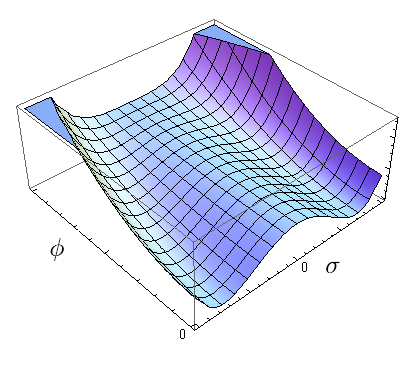
\includegraphics[width=7cm]{Figures/hybridpotential}
%     \caption{The potential $V(\phi,\sigma)$ of hybrid inflation.}
% \end{figure}

The curvature of the potential with respect to $\sigma$ is given by $M_\sigma^2(\phi) \equiv g^2\phi^2 - M^2$; so if $\phi$ starts out much larger than the critical value $\phi_c \equiv M/g$, then the curvature in $\sigma$ is positive and correspondingly large.  In such cases, the system quickly settles to the local minimum at $\sigma = 0$, marking the floor of the super-critical {\it inflationary valley}.  
% In this regime, the hybrid model behaves effectively as a single-field quadratic model, resembling old inflation with an additional vacuum term.  
The potential \eqref{pot} is then
\begin{equation} V(\phi,0) = \frac12 m^2 \phi^2 + \frac{M^4}{4\lambda} = \frac12 m^2 \left( \phi^2 + \aaa^2 \right), \label{valley} \end{equation}
where $\aaa^2 \equiv M^4/2\lambda m^2$ .
% and $M_P \equiv (8\pi G)^{-1/2}$ is the reduced Planck mass.  
(Here we work in Planck units where $M_P \equiv (8\pi G)^{-1/2} = 1$.)
% (Here we introduce an overline notation, indicating that the overlined quantity 
% is expressed in natural units, with $M_P = 1$:
% has been made dimensionless by adding or removing powers of $M_P$: 
% $m \equiv m/M_P$, $\phi \equiv \phi/M_P$, $\widebar V \equiv V/M_P^4$, etc.)
The slow roll evolution of the initially large $\phi$ field is interrupted by a symmetry-breaking phase transition at $\phi = \phi_c$, after which the curvature in $\sigma$ becomes negative.  
The system then rapidly rolls down to one of the two global minima at $\phi=0,\;\sigma=\pm M/\sqrt{\lambda}$.  If $ M^3 \ll \sqrt{\lambda} g m$, then inflation ends within one $e$-folding of expansion after reaching $\phi_c$.
The following parameter values offered in \cite{linde1994hybrid} result predictions that agree with observed features of the scalar density perturbation spectrum: 
% \[ M \sim 10^{11} \text{ GeV} \qquad m \sim 10^2 \text{ GeV} \qquad g^2 \sim \lambda \sim 0.1 \]
\[ M \sim 10^{-8} M_P, \quad m \sim 10^{-17} M_P, \quad g^2 \sim \lambda \sim 0.1 \]

% The regimes are denoted by the relation of $\phi$ to the dimensionless parameter $a \equiv M^4/2\lambda m^2$.  For $\phi \gg a$, the potential is mass dominated; for $\phi \ll a$, it is vacuum dominated.

% \subsubsection{Density Perturbations}

% \begin{enumerate}[label=\arabic{*}.]
% \item $ Q_s = \dfrac{V^{3/2}}{\pi \sqrt{75} \, M_P^3 \, m^2 \phi } = (1.945 \pm 0.052) \times 10^{-5} $
% \item $ n_s - 1 = \dfrac{2 m^2}{V} \left( 1 - \dfrac{3 \, m^2 \phi^2}{2 V} \right) M_P^2 = -0.047 \pm 0.016 $
% \item $ \alpha_s = \dfrac{4 m^4 \phi^2}{V^2} \left( \dfrac{2 m^2}{V} - \dfrac{ 3 m^4 \phi^2}{2 V^2} \right) M_P^4 = -0.040 \pm 0.027 $
% \end{enumerate}

% \paragraph{Number of e-foldings}

Let us assume that inflation ends so abruptly when $\phi$ reaches the critical value $\phi_c$ from above.  The number of $e$-foldings of inflation, $N$, elapsed between the imprinting of CMB density perturbations and the end of inflation must be between 50 and 60, with 55 being an acceptable figure for our purposes.  
% We will find it useful to parameterize the trajectory of the homogeneous $\phi$ field in terms of the number of e-foldings remaining until the end of inflation.
% Reversing the integral expression for $N$ yields a differential equation for $\phi(N)$:
% \[ \ddx{\phi}{N} = \frac{ 2 \phi }{ \phi^2 + \aaa^2 } \]
The initial value $\phi_0$ from which the descent to $\phi_c$ produces $N$ $e$-folds of inflation is then
\begin{equation} \phi_0^2(N) = \aaa^2 \, W \left[ \frac{\phi_c^2}{\aaa^2} \exp \left(\frac{ 4 N + \phi_c^2 }{\aaa^2} \right) \right], \end{equation}
where $W(z)$ is the product logarithm (defined such that $\phi_0(0) = \phi_c$).  
For $\phi_c < M_P$, there exists a threshold near $N \sim \aaa^2$ at which $\phi_0(N)$ changes from $\ll M_P$ to $> M_P$, as shown in Figure \ref{phi_vs_N_a}.  




Since the potential $V(\phi,\sigma)$ exhibits no false vacua, we are left with the possibilities of stochastic and topological eternal inflation. 

\subsubsection{Stochastic Eternal Inflation}

% If eternal inflation is found to occur for field values not far outside the range from which density perturbations are likely to have been imprinted, then it would be difficult to argue that eternal inflation is generically absent from the model.

When restricted to the inflationary valley, the stochastic eternal inflation criterion \eqref{seic} becomes 
\begin{equation} m^2 \phi \lesssim 0.15 \, V^{3/2}. \label{hybrid_seic} \end{equation}
% where $M_P = (8\pi G)^{-1/2}$ is the reduced Planck mass.
where $V = V(\phi,0)$ takes the form \eqref{valley}.

% It is useful to identify two regimes of approximation, in which the potential is dominated by either the quadratic term, $\frac12 m^2\phi^2$ ($\phi \gg \aaa$), or the vacuum term, $M^4/4\lambda$ ($\phi \ll \aaa$).
% \begin{enumerate}
% \item the quadratic term, $\frac12 m^2\phi^2$ ($\phi \gg a$), or
% \item the vacuum term, $\frac1{4\lambda} M^4$ ($\phi \ll a$).
% \end{enumerate}

% By combining the following conditions, we find the constraints under which eternal inflation is allowed.
% \begin{enumerate}
% \item Slow roll conditions
%     \begin{enumerate}[label=\arabic{*}.]
%     \item $\epsilon_\phi = \dfrac{m^4\phi^2}{2V^2} \ll M_P^{-2}$
%     \item $\eta_\phi = \dfrac{m^2}{V} \ll M_P^{-2}$
%     \end{enumerate}
% \item Criterion for eternal inflation: $\phi \lesssim \dfrac{\widebar V^{3/2}}{m^2} \dfrac{M_P}{6.64} $
% \item Observed spectrum of density perturbations
%     \begin{enumerate}[label=\arabic{*}.]
%     \item 
% $ Q_s = \dfrac{V^{3/2}}{\pi \sqrt{75} \, M_P^3 \, m^2 \phi } = (1.945 \pm 0.052) \times 10^{-5} $
%     \item $ n_s - 1 = \dfrac{2 m^2}{V} \left( 1 - \dfrac{3 \, m^2 \phi^2}{2 V} \right) M_P^2 = -0.047 \pm 0.016 $
%     \item $ \alpha_s = \dfrac{4 m^4 \phi^2}{V^2} \left( \dfrac{2 m^2}{V} - \dfrac{ 3 m^4 \phi^2}{2 V^2} \right) M_P^4 = -0.040 \pm 0.027 $
%     \end{enumerate}
% \end{enumerate}
% $ \alpha_s = \dfrac{4 m^4 \phi^2}{V^2} \left( \dfrac{2 m^2}{V} - \dfrac{ 3 m^4 \phi^2}{2 V^2} \right) M_P^4 = -0.040 \pm 0.027 $
% \paragraph{Quadratic Approximation}%: $V(\phi,0) \approx \dfrac12 m^2 \phi^2$}

In the \textbf{quadratic approximation} $\phi \gg \aaa$, the inflaton behaves like a free field with mass $m$.  The slow roll conditions are satisfied when $\phi \gg 1$, and the criterion for eternal inflation is \[ \phi \gtrsim 4.3 \, m^{-1/2}.\] %Q_s \gtrsim 0.24 \]
In the regime $\phi_c \lesssim 1$, the value of $\phi$ at 55 e-foldings before the end of inflation asymptotes to approximately $14.83 \, M_P$ as $\aaa \to 0$.  Values of $\aaa$ larger than $\mathcal O(1)$ are excluded by measurements of the spectral index $n_s$.
For $m \ll 1$ and $\phi_c \lesssim 1$, the field cannot satisfy the eternal inflation criterion within $10^{10}$ $e$-folds.
The parameters of the perturbation spectrum for $\phi \approx 14.8 \, M_P$ are given in Table \ref{quadtable}.
% { \def\arraystretch{2.1}
% \begin{table}[h]
% \centering
% % \begin{tabular}{ccll}
% %                 & Expression & $\phi \approx 14.8$ & Measured Value \\
% %     $Q_s$       & $\dfrac{m \phi^2} {2\pi\sqrt{150}}$  &  $\phantom{-}2.8 \, m$  &  $(1.945 \pm 0.052) \times 10^{-5}$
% % \\  $n_s - 1$   & $-8\,\phi^{-2}$               & $-0.036$         & $-0.047 \pm 0.016$
% % \\  $\alpha_s$  & $-32\,\phi^{-4}$              & $-0.00067$       & $-0.040 \pm 0.027$
% % \\  $r$         & $\phantom-64\,\phi^{-2}$      & $\phantom-0.29$  & $\phantom-0.2^{+0.07}_{-0.05}$
% % \end{tabular} 
% \begin{tabular}{ccll}
%                 & $\phi \approx 14.8$ & Measured Value \\
%     $Q_s$       &  $\phantom{-}2.8 \, m$  &  $(1.945 \pm 0.052) \times 10^{-5}$
% \\  $n_s - 1$   & $-0.036$         & $-0.047 \pm 0.016$
% \\  $\alpha_s$  & $-0.00067$       & $-0.040 \pm 0.027$
% \\  $r$         & $\phantom-0.29$  & $\phantom-0.2^{+0.07}_{-0.05}$
% \end{tabular} 
% \caption{Parameters of the density perturbation spectrum in the quadratic approximation.}
% \label{quadtable}
% \end{table} }

% \[ Q_s \approx \dfrac{ m \phi^2} {2\pi\sqrt{150} M_P^3} \approx 2.8 m \approx (1.945 \pm 0.052) \times 10^{-5} \]
% \[ n_s - 1 \approx -\dfrac{8 M_P^2}{\phi^2} \approx -0.047 \pm 0.016 \implies \phi_e \approx 13 M_P \]
% \[ \alpha_s \approx -\dfrac{32 M_P^4}{\phi^4} \approx -0.040 \pm 0.027 \implies \phi_e \approx 5 M_P \]
% \[ r = \frac{2^6 M_P^2}{\phi^2} \overset?< 0.30 \impliedby \phi > 15 M_P \]

% \paragraph{Vacuum Approximation}%: $V(\phi,0) \approx \dfrac{M^4}{4\lambda}$ }

In the \textbf{vacuum approximation} $\phi \ll \aaa$, the first and second slow roll conditions are, respectively, $\phi \ll \aaa^2$ and $\aaa^2 \gg 1$; both are easily met.  
The criterion \eqref{hybrid_seic} is then 
\begin{equation} \phi \lesssim 0.053 \, m \, \aaa^3. \label{hybrid_vacuum_seic} \end{equation}
Given $m \ll 1$ and $\aaa \gg 1$, this too is easily satisfied, meaning that eternal inflation occurs for small field inflation in the vacuum dominated regime with $\sigma = 0$.
For $\phi > \phi_c$, \eqref{hybrid_vacuum_seic} implies a lower bound on the scalar density perturbation amplitude,
% \[ a \gg \phi_c \qquad a^2 \gg \phi_c \qquad a^3 \gtrsim \dfrac{\phi_c}{m} \]
$ Q_s \gtrsim 0.25 $, %4 \times 10^{-3} $
that is larger than the measured value by four orders of magnitude.
Hence density perturbations must have been imprinted at $\phi < \phi_c$.  Not accounting for the effects of departure of $\sigma$ from $0$, the amplitude would match observations for $\phi \approx 2.2 \times 10^{-5} \, \phi_c$.

In the regime $\aaa \gg 1$, 55 e-foldings affects almost no change in the field, and we can approximate $\phi_0 \approx \phi_c$.  
The parameters of the perturbation spectrum are given in Table \ref{vactable}.

% { \def\arraystretch{2.5}
% \begin{table}[h]
% \centering
% \begin{tabular}{ccll}
%                 & $\phi \approx \phi_c$ & Measured Value \\
%     $Q_s$       & $\dfrac{1} {2\pi\sqrt{150}} \dfrac{m \, \aaa^3}{\phi_c}$  &  $(1.945 \pm 0.052) \times 10^{-5}$ \\
%     $n_s - 1$   & $\dfrac{1}{\aaa} \left( 1 - \dfrac{12 \phi_c^2}{\aaa} \right)$  &  $-0.047 \pm 0.016$ \\
%     $\alpha_s$  & $\dfrac{2^{4} \phi_c^2}{\aaa^6} \left(1 - \dfrac32 \dfrac{\phi_c^2}{\aaa^2} \right) $                   & $-0.040 \pm 0.027$ \\
%     $r$         & $\dfrac{32 \, \phi_c^2}{\aaa^2}$  & $\phantom-0.2^{+0.07}_{-0.05}$
% \end{tabular} 
% \caption{Parameters of the density perturbation spectrum in the vacuum approximation.}
% \label{vactable}
% \end{table} }

The slow roll conditions for $\sigma$ in the vacuum approximation are
\[ \lambda \widebar\sigma \abs{\eta^2 - \widebar\sigma^2} \ll m^2 \aaa^2 \quad\text{and}\quad \lambda \abs{\eta^2 - 3\widebar\sigma^2} \ll m^2 \aaa^2,\]
where $\eta \equiv M/\sqrt{\lambda}$.
\[ Q_s \approx \dfrac{g} {8\pi\sqrt{75} \, \lambda^{3/2}} \dfrac{ M^5 }{ m^2 } \approx (1.945 \pm 0.052) \times 10^{-5} \]
% \[ n_s - 1 \approx \dfrac{2\lambda m^2}{M^4} \left( 1 - \dfrac{24 \lambda m^2}{g^2 M^2} \right) \approx -0.047 \pm 0.016 \]
% \[ \alpha_s \approx \dfrac{2^{10} \lambda^3}{g^2} \dfrac{m^6}{M^{10}} \left(1 - \dfrac{3 \lambda }{2 g^2} \dfrac{m^2}{M^2} \right) \approx -0.040 \pm 0.027 \]
% \[ r = \frac{2^8 \lambda^2 M_P^2 \, m^4 \phi^2}{M^8} \overset?< 0.30 \impliedby \phi < \frac{M^4}{m^2} \frac{M_P}{30\lambda} \]

% \paragraph{Number of e-foldings}

% The number of $e$-folds of inflation, $N$, elapsed since the imprinting of CMB density perturbations is between 50 and 60, with 55 being an acceptable figure.  
% Reversing the integral expression for $N$ yields a differential equation for $\phi(N)$:
% \[ \ddx{\phi}{N} = \frac{ 2 \phi }{ \phi^2 + \aaa^2 } \]
% The initial value $\phi_0$ from which the descent to $\phi_c$ produces $N$ $e$-folds of inflation is given by
% \[ \phi_0^2(N) = \aaa^2 \, W \left[ \frac{\phi_c^2}{\aaa^2} \exp \left(\frac{ 4 N + \phi_c^2 }{\aaa^2} \right) \right], \]
% where $W(z)$ is the product logarithm (defined such that $\phi_0(0) = \phi_c$).  
% For any $\phi_c < M_P$, there exists a threshold near $N \sim \aaa^2$ at which $\phi_0(N)$ changes from $\ll M_P$ to $> M_P$, as shown in the figure below.  

We see that for $\aaa < 1$, eternal inflation is inevitable as the number of elapsed e-foldings balloons to the values larger than $\sim 10^6$.  There also appears to be a region of parameter space near $\aaa \sim 1$ where eternal inflation occurs in the vacuum dominated regime.  In this region, we must consider the effects of the $\sigma$ field departing from zero as the system falls toward one of the local minima.  We must also take into account topological eternal inflation near the saddle point, as the field in neighboring regions of space may fall toward different vaccuum values.
% When $\phi \gtrsim a$, $\phi$ becomes linear in $a$ and $N$.

% \begin{figure}[h]
%     \centering
%     \subfigure[$\phi_0$ versus $a^2$ and $N$ with $\phi_c = 10^{-7}$.]{
\includegraphics[width=8cm]{phi0_vs_a_N_3d}}
%     \subfigure[$\phi_0(N)$ with $a \in \{0.1,\,1,\,10,\,100\}$ (left to right).]%[Dependence of $\phi_0(55)$ on $\phi_c$ with $a = 0.01$.]
%     {
\includegraphics[width=8cm]{phi0_vs_N}}
% \end{figure}

\begin{figure}[h]
    \centering
    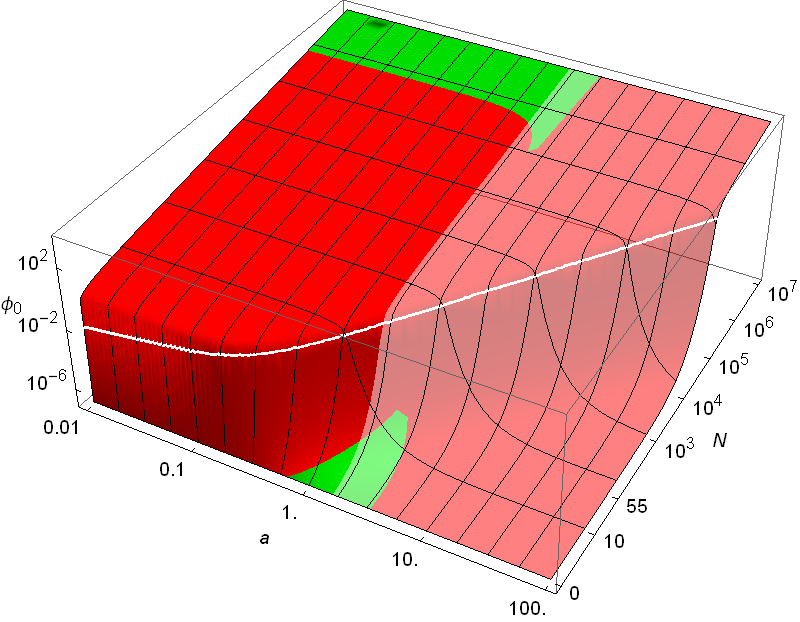
\includegraphics[width=7.5cm]{Figures/phi0_vs_a_N_Eternal_Region}
    \caption{A plot of $\phi(N;\aaa)$, the field value as a function of the number of e-foldings $N$ until the end of inflation and the paramter $\aaa$.  The green shaded regions are those in which stochastic eternal inflation occurs.  The greyed out region is excluded by the constraing on the scalar index $n_s$.  The white line marks the boundary between quadratic and vacuum approximations at $\phi = \aaa$.}
    \label{phi_vs_N_a}
\end{figure}

% \begin{figure}[h]
%     \centering
%     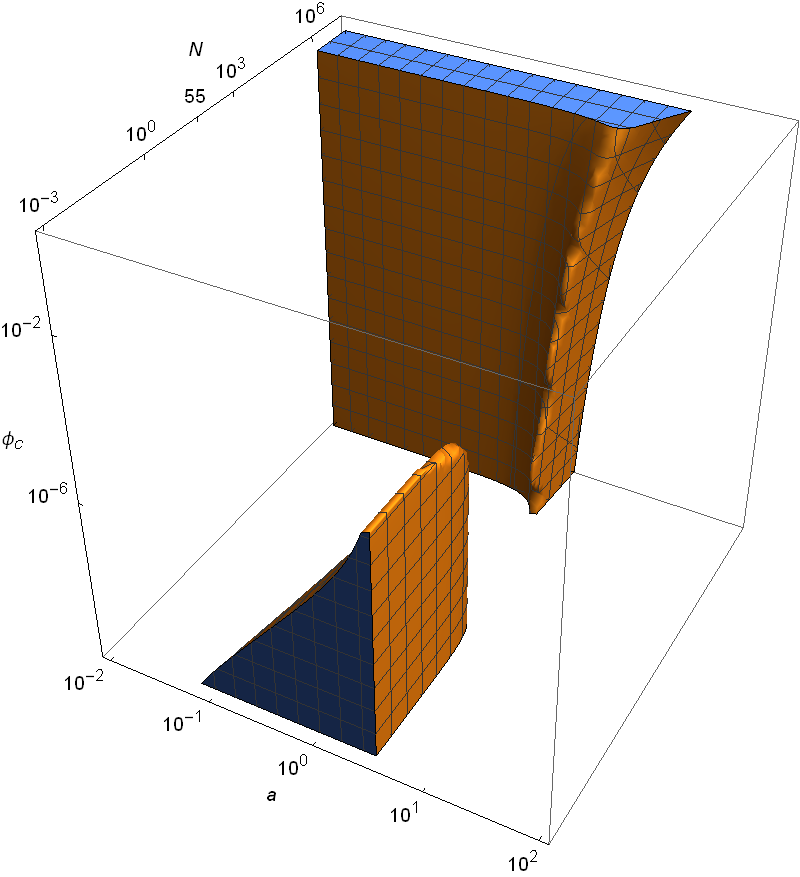
\includegraphics[width=7.5cm]{Figures/RegionPlot_a_N_phi0}
% \end{figure}

\subsubsection{Topological Eternal Inflation}

For $\phi < \phi_c$, the potential has two local minima at $\pm M/\sqrt{\lambda}$.  
In neighboring regions of space that begin with $\sigma$ near its local maximum, the field can roll down the slope in different directions -- toward $-M/\sqrt{\lambda}$ or $+M/\sqrt{\lambda}$.  
This leads to the formation a domain wall in which the field is stuck near the local maximum.  
If the potential near the maximum is sufficiently flat, so that the domain wall thickness exceeds the Hubble radius, then the volume within the wall will inflate faster than it decays, resulting in eternal inflation.
\[ \left. \ddx{^2V}{\sigma^2} \right\rvert_{\sigma=0} \ll \frac{V}{3 M_P^2} \]
\[ g^2 \phi^2 - M^2 \ll \frac{1}{3 M_P^2} \left( \frac{M^4}{4\lambda} + \frac{m^2}{2} \phi^2 \right) \]
\[ \left( g^2 - \frac{4\pi}{3} \, m^2 \right) \phi^2 \ll \left( 1 + \frac{2\pi}{3} \frac{M^2}{\lambda} \right) M^2 \]
If $m \ll 1$ and $M^2 \ll \lambda$, then the potential is sufficiently flat for $\phi \ll \phi_c$.  

We must also assert that the kinetic energy of $\phi$ be sub-dominant -- satisfying the slow roll conditions.  The two can be consistent if the potential is vacuum dominated:
\[ \phi \ll \frac{M^4}{m^2} \frac{M_P}{\lambda} \qquad M^4 \gg \lambda m^2 \]

\[m = 1 \quad m = 10^{-5} \quad m = 10^{-10} \]

\[ \log_{10} \frac{\phi_0}{a} = 0 \quad \log_{10} \frac{\phi_0}{a} = -2 \quad \log_{10} \frac{\phi_0}{a} = 4 \]


    % \[ n_s - 1 = \dfrac{2 m^2}{V} \left( 1 - \dfrac{3 \, m^2 \phi^2}{2 V} \right) M_P^2 = -0.047 \pm 0.016 \]
    % \[ \alpha_s = \dfrac{4 m^4 \phi^2}{V^2} \left( \dfrac{2 m^2}{V} - \dfrac{ 3 m^4 \phi^2}{2 V^2} \right) M_P^4 = -0.040 \pm 0.027 \]


